\documentclass[conference]{IEEEtran}
\makeatletter
\def\ps@headings{%
\def\@oddhead{\mbox{}\scriptsize\rightmark \hfil \thepage}%
\def\@evenhead{\scriptsize\thepage \hfil \leftmark\mbox{}}%
\def\@oddfoot{}%
\def\@evenfoot{}}
\makeatother
\pagestyle{headings}

\hyphenation{op-tical net-works semi-conduc-tor}


\usepackage{subfigure}
\usepackage{soul}


\usepackage{listings}
\usepackage{color}

\definecolor{dkgreen}{rgb}{0,0.6,0}
\definecolor{gray}{rgb}{0.5,0.5,0.5}
\definecolor{mauve}{rgb}{0.58,0,0.82}

\lstset{frame=tb,
	language=Java,
	aboveskip=3mm,
	belowskip=3mm,
	showstringspaces=false,
	columns=flexible,
	basicstyle={\small\ttfamily},
	numbers=none,
	numberstyle=\tiny\color{gray},
	keywordstyle=\color{blue},
	commentstyle=\color{dkgreen},
	stringstyle=\color{mauve},
	breaklines=true,
	breakatwhitespace=true,
	tabsize=3
}

\usepackage{algorithmic}
\usepackage[ruled,vlined]{algorithm2e}
\usepackage{graphicx}


\if CLASSINFOpdf
  \usepackage[pdftex]{graphicx}
  % declare the path(s) where your graphic files are
  % \graphicspath{{../pdf/}{../jpeg/}}
  % and their extensions so you won't have to specify these with
  % every instance of \includegraphics
  % \DeclareGraphicsExtensions{.pdf,.jpeg,.png}
\else
  % or other class option (dvipsone, dvipdf, if not using dvips). graphicx
  % will default to the driver specified in the system graphics.cfg if no
  % driver is specified.
  % \usepackage[dvips]{graphicx}
  % declare the path(s) where your graphic files are
  % \graphicspath{{../eps/}}
  % and their extensions so you won't have to specify these with
  % every instance of \includegraphics
  % \DeclareGraphicsExtensions{.eps}
\fi
% graphicx was written by David Carlisle and Sebastian Rahtz. It is
% required if you want graphics, photos, etc. graphicx.sty is already
% installed on most LaTeX systems. The latest version and documentation can
% be obtained at:
% http://www.ctan.org/tex-archive/macros/latex/required/graphics/
% Another good source of documentation is "Using Imported Graphics in
% LaTeX2e" by Keith Reckdahl which can be found as epslatex.ps or
% epslatex.pdf at: http://www.ctan.org/tex-archive/info/
%
% latex, and pdflatex in dvi mode, support graphics in encapsulated
% postscript (.eps) format. pdflatex in pdf mode supports graphics
% in .pdf, .jpeg, .png and .mps (metapost) formats. Users should ensure
% that all non-photo figures use a vector format (.eps, .pdf, .mps) and
% not a bitmapped formats (.jpeg, .png). IEEE frowns on bitmapped formats
% which can result in "jaggedy"/blurry rendering of lines and letters as
% well as large increases in file sizes.
%
% You can find documentation about the pdfTeX application at:
% http://www.tug.org/applications/pdftex


\title{Titolo del progetto svolto}

% Author names 
% note positions of commas and nonbreaking spaces ( ~ ) LaTeX will not break
% a structure at a ~ so this keeps an author's name from being broken across
% two lines.
% use \thanks{} to gain access to the first footnote area
% a separate \thanks must be used for each paragraph as LaTeX2e's \thanks
% was not built to handle multiple paragraphs
\author{
Nome Autore1\IEEEauthorrefmark{1},
Nome Autore2\IEEEauthorrefmark{1},
\\
\IEEEauthorblockA{\IEEEauthorrefmark{1} DISI, University of Bologna, Italy \\
 \\
Emails: autore1@email.it, autore2@email.it, autore3@email.it}}


\begin{document}

% make the title area
\maketitle


% The Abstract
\begin{abstract}
Riassumi qui il succo del progetto, in 20-30 righe.

\end{abstract}



\section{Introduction}
Descrivi qui il contesto generale, i contributi del progetto, e la struttura del documento.
 

\section{Related works}
Fornisci una breve rassegna di articoli di ricerca, software, prototipi o tecnologie che sono collegate in qualche modo al problema affrontato nel progetto. Tutti i lavori devono essere referenziati ed inseriti nella Bibliografia.

\section{Architecture}
Il sistema \'e stato sviluppato in modo da poter girare su dispositivi Android, lasciando in questo modo la possibilità di essere utilizzato in larga scala e senza costi aggiuntivi al prezzo del dispositivo stesso.
Suddetto applicativo è costituito da due tipologie di layer applicativi che potremmo denominare Publisher e Observer così da poter rendere il pi\'u intuitivo possibile il ruolo da loro ricoperto.
\begin{figure}[h!]
	\centering
	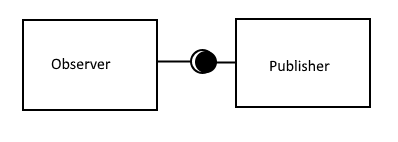
\includegraphics[width=0.7\linewidth]{ps}
	\caption{Ruoli}
	\label{fig:ps}
\end{figure}
Il ruolo del Publisher viene assunto da tutti i dispositivi in possesso ai pedoni. Il loro compito principale \'e quello di avvisare i veicoli circostanti riguardo la propria posizione corrente.
Tutti i veicoli presenti sulla strada, invece, sono Observer ed hanno l'obbligo di ascoltare in ogni istante i Publisher, elaborare i loro dati ed avvertire il conducente.
La struttra della rete risulta dunque essere un miscuglio approsimatamente omogeneo di Publisher ed Observer.
\begin{figure}[h!]
	\centering
	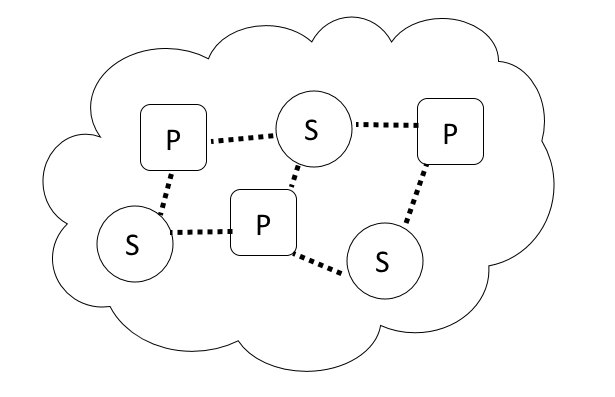
\includegraphics[width=0.7\linewidth]{net}
	\caption{Rete Omogenea}
	\label{fig:net}
\end{figure}
La forza di questo sistema è il fatto che la rete non preveda una vera e propria sturuttra, ma che si adatti a quelle che sono le limitazioni dell'ambiente circostante.
Questa qualità del sistema lo rende flessibile e particolarmente scalabile.

\section{Implementation}
Descrivi come e\' stato implementato il sistema, ossia tecnologie utilizzate, linguaggi, APIs, etc. Nel caso, fornisci pseudo-codice degli algoritmi
piu\' interessanti sviluppati nel progetto.

\subsection{Ambiente di Sviluppo}
Come gi\'a descritto in precedenza, il sistema \'e stato completamente sviluppato per sistema operativo Android in modo da consentire la maggior portabilit\'a del software.
Infatti il nostro obiettivo non era solo la verifica verticale delle funzionalit\'a del software, ma anche il confronto orizzontale tra dispositivi che utilizzano hardware differenti. Questo ha consentito di trovare i punti in comune ma anche le discrepanze tra i diversi hardware e di generare un software flessibile in grado di adattarsi al dispositivo host.
Per lo sviluppo e\' stato utilizzato l'IDE di default di Android ovvero Android Studio con linguaggio di programmazione Java.


\subsection{Obiettivi}
L'idea iniziale era quella di riuscire ad inidividuare un pedone con il maggior preavviso possibile, ma limitando il consumo energetico del dispositivo ad egli in possesso.
Per fare cio\' abbiamo effettuato alcuni test utilizzando il Bluetooth, la tecnologia\' a radio frequenza con il miglior risparmio energetico. In particolare ci siamo concentrati sull'utilizzo dei Beacon Bluetooth inviati dal dispositivo pedone ed elaborati dal veicolo.
Al loro interno sono stati inseriti dati fittizi che simulassero un payload di dimensioni verosimili.
Le prove effettuate includevano l'invio dei beacon sia dal veicolo in movimento che dal pedone a velocita\' ridotta.
Purtroppo in entrambi casi i risulati ottenuti sono notevolmente scadenti. Infatti i dispositivi riuscivano a trovarsi solo a distanze quasi nulle (non piu\' di una decina di metri).
La nostra seconda scelta e\' dunque ricaduta sull'utilizzo del WiFi Direct(P2P). Nel paragrafo seguente vedremo in breve come funziona questo standard.


\subsection{WiFi Direct e Problemi riscontrati}
Wi-Fi Direct (nato con il nome Wi-Fi P2P - Wi-Fi Peer-to-Peer) è uno standard della Wi-Fi Alliance, ormai comune in molti prodotti, come smartphone, tablet, stampanti, videocamere digitali, console di gioco e scanner, che consente a due o più dispositivi certificati di connettersi tra loro con un collegamento Wi Fi diretto senza aver bisogno di un router wireless o di un hotspot.
In particolare questa tecnologia prevede 3 fasi prima dio poter scambiare dati:
\\
1) Effettuare il discovery dei dispositivi circastanti
\\
2) Creazione di un gruppo (se questo non esiste gia') al fine di poter poi accettare connesione
\\
3) Effettuare handshake di connessione
\\
Come racconta lo standar IEEE, il WiFi P2P garantisce una riuscita della connessione all'interno del range dei 13 secondi. Purtroppo, per il nostro applicativo queste latenze sarebbero state enormi ed avrebbero reso il sistema inutilizzabile.
Abbiamo dunque deciso di sviluppare un applicazione di chat base, che ci aiutasse a stimare il reale tempo di riuscita della connessione tra due dispositivi.
I test ci hanno riportato quanto segue:
\\
- Tempo di connessione ~3/4,\\
- Una volta stabilita la connessione il tempo di risposta ad un messaggio era pressoche\' nullo.
I 3-4 di connessione non rispecchiavano in tutto per tutto le nostre esigenze in quanto, non certi del range del segnale WiFi, 3s * (50km/h / 3.6) =~40m di range sarebbero stati persi in partenza.
Non potendo consentire la connessione tra i dispositivi, ci rimaneva unicamente la fase di Discovery da sfruttare.
All'interno del record di Discovery, infatti, vi si puo\' inserire qualunque dato sottoforma di tabella hash ed il processo di segnalazione e di ricezione del segnale e\' pressoche\' immediato.
Fatte queste considerazioni, abbiamo deciso di demolire l'applicazione di chat lasciando unicamente la parte di discovery ed effettuare svariati test in cui misuravamano la distanza minima in cui i due dispositivi riuscivano a vedersi per la prima volta.
I riusultati sono stati eccezionali. Infatti i valori in metri ottenuti sono stati da un centinaio di metri in campo aperto a 45-50 metri in curva con traiettoria in linea d'aria offuscata da ostacoli.
Questo principio e\'risultato per noi essere le fondamenta vere e proprie del sistema stesso.
Sfortunatamente le librerie di android non funzionano molto bene per quanto riguarda il publishing ed il discovery nel WiFi Direct. Infatti se si vuol pubblicare i propri dati sulla rete bisogna anche effettuare un'operazione continua di Discovery, altrimenti nessuno dato viene spedito. Inoltre (considerando che il Discovery chiama una callback ogni volta che trova un dispoositivo) la callback del Discovery non segnala lo stesso dispositivi piu\' di una volta se esso e\' gia\' stato trovato anche se possiede un record differente.
Questo ci ha costretti a resettare la procedura del discovery ogni T secondi in modo da poter mettere il dispositivo Observer nuovamente in ascolto anche di Pubblisher gia\' trovati.
Per valori di T inferiori ai 7-8 secondi si rischia di mandare in crash il driver del modulo WiFi che, non so se per problemi interni o per verifiche di funzionamento del sistema operativo, viene disattivato bloccando qualsiasi forma di ricezione e/o trasmissione.
L'applicativo lato publisher fornisce all'interno del proprio record di service discovery i seguenti dati che varro poi discussi nei paragrafici successivi nei relativi modelli.
- Longitudine\\
- Latitudine\\
- Velocita\\
- Timestamp\\
- Timestamp della Posizione\\
- Accuratezza\\
- Bearing\\
Lato Observer invece, i dati di tutti i pedoni trovati tramite il discovery vengono salvati(eventualmente aggiornati se gia trovati in precedenza), processati ed alla fine del loro ciclo vita eliminati.


\subsection{Modello di Previsione}
Questo modello viene implementato lato Observer e si occupa di elaborare i dati ricevuti dai diversi Publisher ed incrociarli con quelli del veicolo che rappresenta.
Un modello di previsione prevede come input il tragitto che il veicolo dovra percorrere sottofroma di Polilinea (vettore di segmenti) ed un gestore di posizionamento che sfrutti il segnale GPS in modo da sapere in ogni istante le cordinate attuali del veicolo.
Dati questi input, per ogni Publisher trovato stima se in un tratto della Polilinea di input il veicolo potrebbe andare a collidere con il Publisher. Nel caso lo segnala sulla mappa.
La stima di collisione viene effettuata utilizzando il seguente algoritmo.
 
 
\begin{figure}[h!]
	\centering
	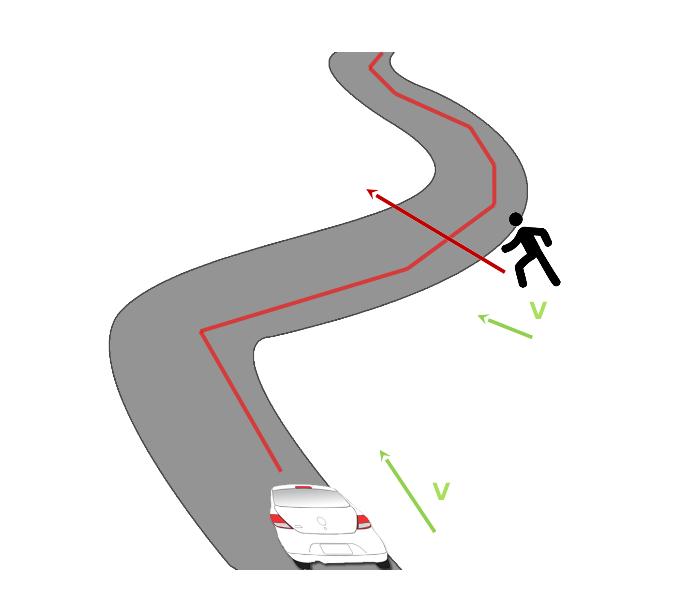
\includegraphics[width=0.7\linewidth]{prevmod}
	\caption{Modello di Previsione}
	\label{fig:prevmod}
\end{figure}
 
Il concetto di fondo e\' che l'uomo collidera\' con il veicolo solo se la sua traiettoria e la sua velocita\' partendo da un punto A lo porteranno in un punto B tale per cui il segmento AB interseziona uno dei tratti della Polilinea realitiva al tragitto del veicolo.
La seguente funzione verifica se due segmenti si intersezionano.

\begin{lstlisting}
/**
* Check if the human will intersect the vehicle
* @param h human service Object
* @return True -> Intersection
*/
public boolean willHumanIntersectVehicle(HumanService h) {
	LatLng loc = getCurrentPosition();
	int start = getCurrentPolylineSegment();
	int end = start;
	// Search indexes on which check intersection
	for(int i = start; i < route.size()-1; i++)
	{
		double d = getPointSegmentProjectionDistance(
			route.get(i),
			route.get(i+1),
			loc);
		if(d < WIFI_MAX_RANGE)
		{
			end = i+1;
		}else{
			break;
		}
	}
	if(end ==  start)
	{
		// All segments are inside 200 meters range
		end = route.size()-1;
	}

	// Intersection check
	for(int i = start; i < end; i++)
	{
		if(doIntersect(
			route.get(i), // P1 of the vehicle
			route.get(i+1), // P2 of the vehicle
			new LatLng(h.latitude, h.longitude), // P1 human
			h.getHumanPositionIn(
			(int) Math.ceil(WIFI_MAX_RANGE / getCurrentSpeed()))  // P2 of the human
		))
		{
		return true;
		}
	}
	return false;       // No intersections
}

\end{lstlisting}
Prima di tutto all'interno di questa funzione viene richiesta la posizione corrente del veicolo ed il segmento di polilinea all'interno del quale esso si trova.
Per trovare il segmento di polilinea corrente (funzione \textit{getCurrentPolylineSegment}), viene effettuato un calcolo trigonometrico della distanza tra la posizione del veicolo ed ogni segmento. Successivamente il tratto con la distanza punto-segmento minore e\' considerato quello corrente.
La distanza punto-segmento in geometria sferica viene calcolata con il seguente algoritmo.
Definiamo con AB il segmento in questione e con C la posizione del veicolo.\\
1) Convertire le coordinate terrestri in coordinate Cartesiane (utilizzando come orgine il centro della terra).\\
2) Calcolare T, il punto sulla retta AB piu\' vicono al  punto C utilizzando i tre seguenti prodotti vettoriali:
\\\\	a) G = A x B\\

	b) F = C x G\\

	c) T = G x F\\

3) Normalizzare T a moltiplicarlo per il raggio della terra.
4) Riconvertire il valore in latitudine e lonfitudine.
5) Verificare che il punto si trovi esattamente sul segmento AB, nel caso sovrfascriverlo con l'estremo del segmento piu\' vicino.
6) Utilizzare la formula della distanza tra due punti in geometria sferica per trovare la distanza punto-segmento.

Proseguento con l'analisi della funzione \textit{willHumanIntersectVehicle}, il primo ciclo for, partendo dal segmento corrente, cerca quali sono i segmenti di polilinea la cui distanza tra segmento e posizione del veicolo risulta essere inferiore al range del WiFi, definito dalla costante WIFI\_MAX\_RANGE. Questo perche\' si presume che il veicolo non possa ricevere un segnale piu\' distante del normale range di trasmissione.
Una volta terminata questa verifica, avremo un estremo superiore ed un estremo inferiore che limitano il numero di indici dei segmenti sui quali poi verra\' eseguito il controllo di intersezione con il segmente pedone.
Il secondo ciclo for esegue per ogni segmento compreso nell intervallo prima definito il controllo di intersezione con il segmento del pedone.
Questo controllo viene eseguito dalla funzione \textit{doIntersect} alla quale vengono passati i due punti del segmento veicolo, la posizione del pedone descritta all'interno del record di Discovery e la stima della posizione del pedone tra J secondi, dove J e\' il tempo impiegato dal veicolo a percorre il range del WiFi.
\textit{doIntersect} e\' l'unica funzione ad utilizzare calcoli euclidei invece che sferici. Questo perche\' la superfice di una sfera per porzioni molto piccole, puo\' essere considerata una superficie piana.
 
 
 

\section{Performance evaluation}
Illustra qui i risultati sperimentali (simulazioni o esperimenti) che catturano le prestazioni del sistema realizzato. Chiarisci quali sono gli indici di stima
e come sono calcolati. Inserisci un breve commento per ogni grafico.

\section{Conclusioni}
Conclusioni, possibili sviluppi futuri e limitazioni del progetto realizzato

%% Inserisci bibliografia dei lavori citati (consiglio l'utilizzo di bibtex)
\bibliographystyle{plain}
\begin{thebibliography}{15}

\bibitem{NomeRiferimento}
\newblock{Lista Autori} 
\newblock{Titolo Lavoro}
\newblock{\textit{Nome Rivista o Convegno}}, pagine, anno pubblicazione.

\end{thebibliography}
\end{document}